\begin{figure}[t]
    \centering
    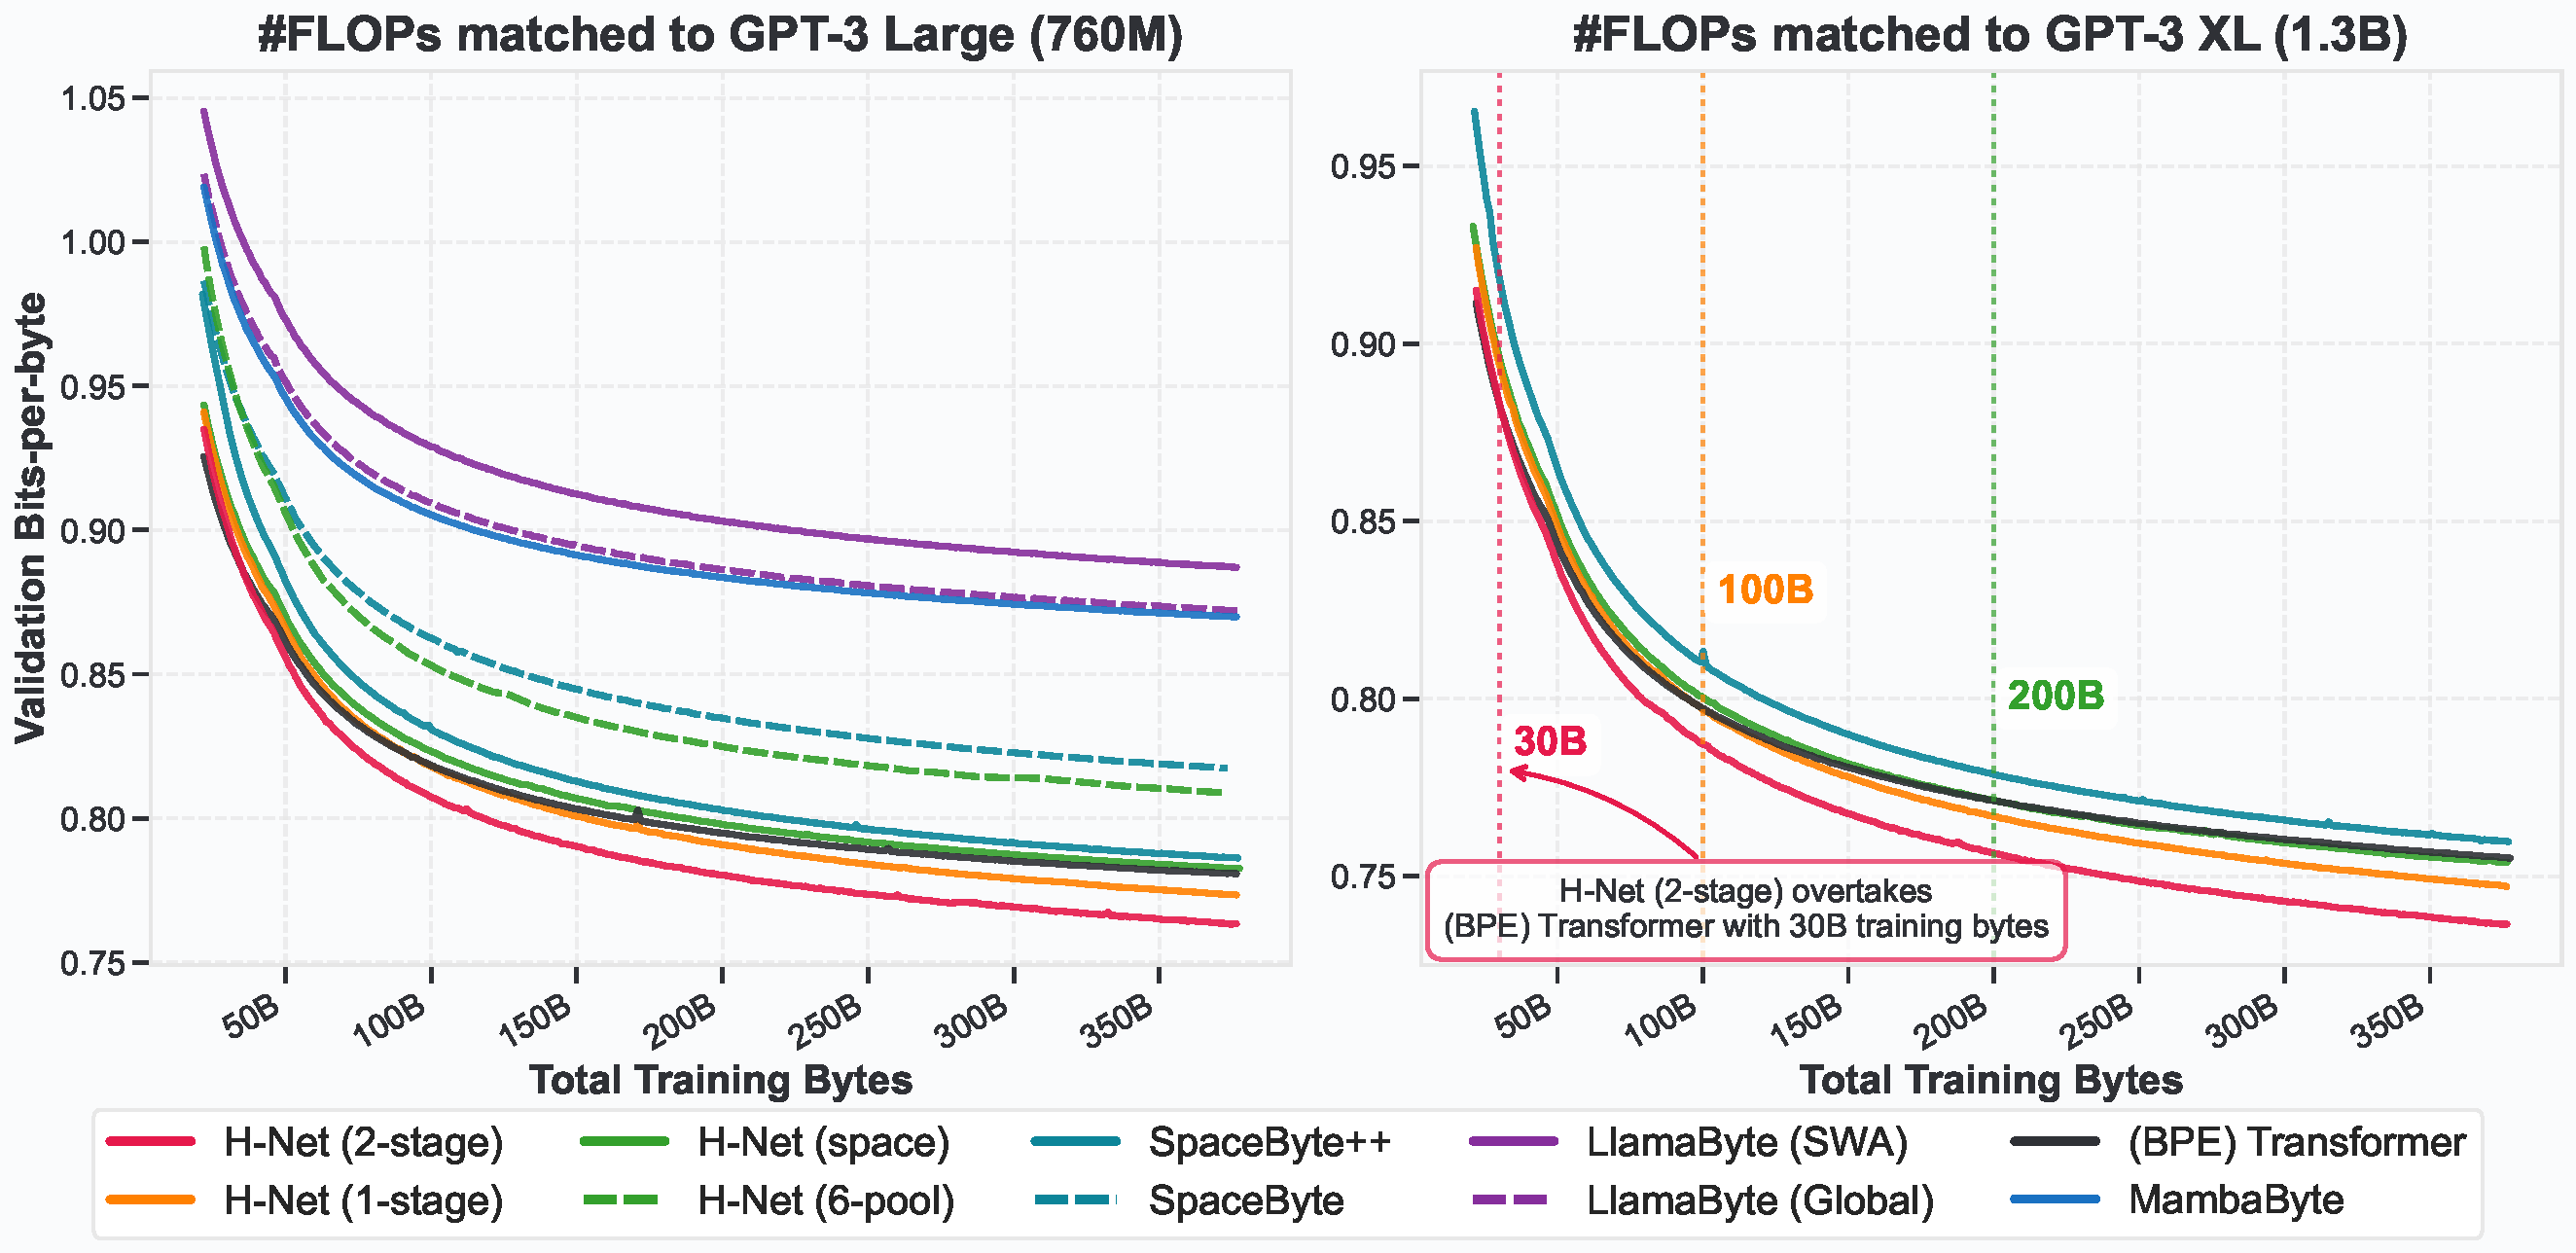
\includegraphics[width=1.0\linewidth]{fig_img/bpb_curve.pdf}
    \caption{
    \textbf{Validation Bits-per-byte (BPB) throughout training} for different models at Large ($760$M, left) and XL ($1.3$B, right) scales with matched computational and data budgets for training.
    All models but Transformer take raw byte inputs (Transformer uses GPT-2 tokenizer).
    Vertical dotted lines indicate crossover points where \model{} begins to outperform Transformer with predefined BPE tokenization.
    From the curves we can clearly see the following: (1) all hierarchical models (\ie{} SpaceByte++, \model{} variants) outperform the isotropic models (\ie{} Transformer, MambaByte, LlamaByte); (2) dynamic chunking is more powerful than BPE tokenizers; and (3) DC is more effective than other chunking strategies.
    Furthermore, \model{}'s \twostage{} variant consistently outperforms \onestage{} across both scales, demonstrating the effectiveness of deeper hierarchies.
    See \cref{tab: architecture} for architectural details.
    }
    \label{fig: bpb_curve}
\end{figure}
